
\section{Ontology Usage}

We chose the Opengroup's Service Oriented Architecture as a 

\subsection{Ontology details}

\begin{figure}[!h]
\centering
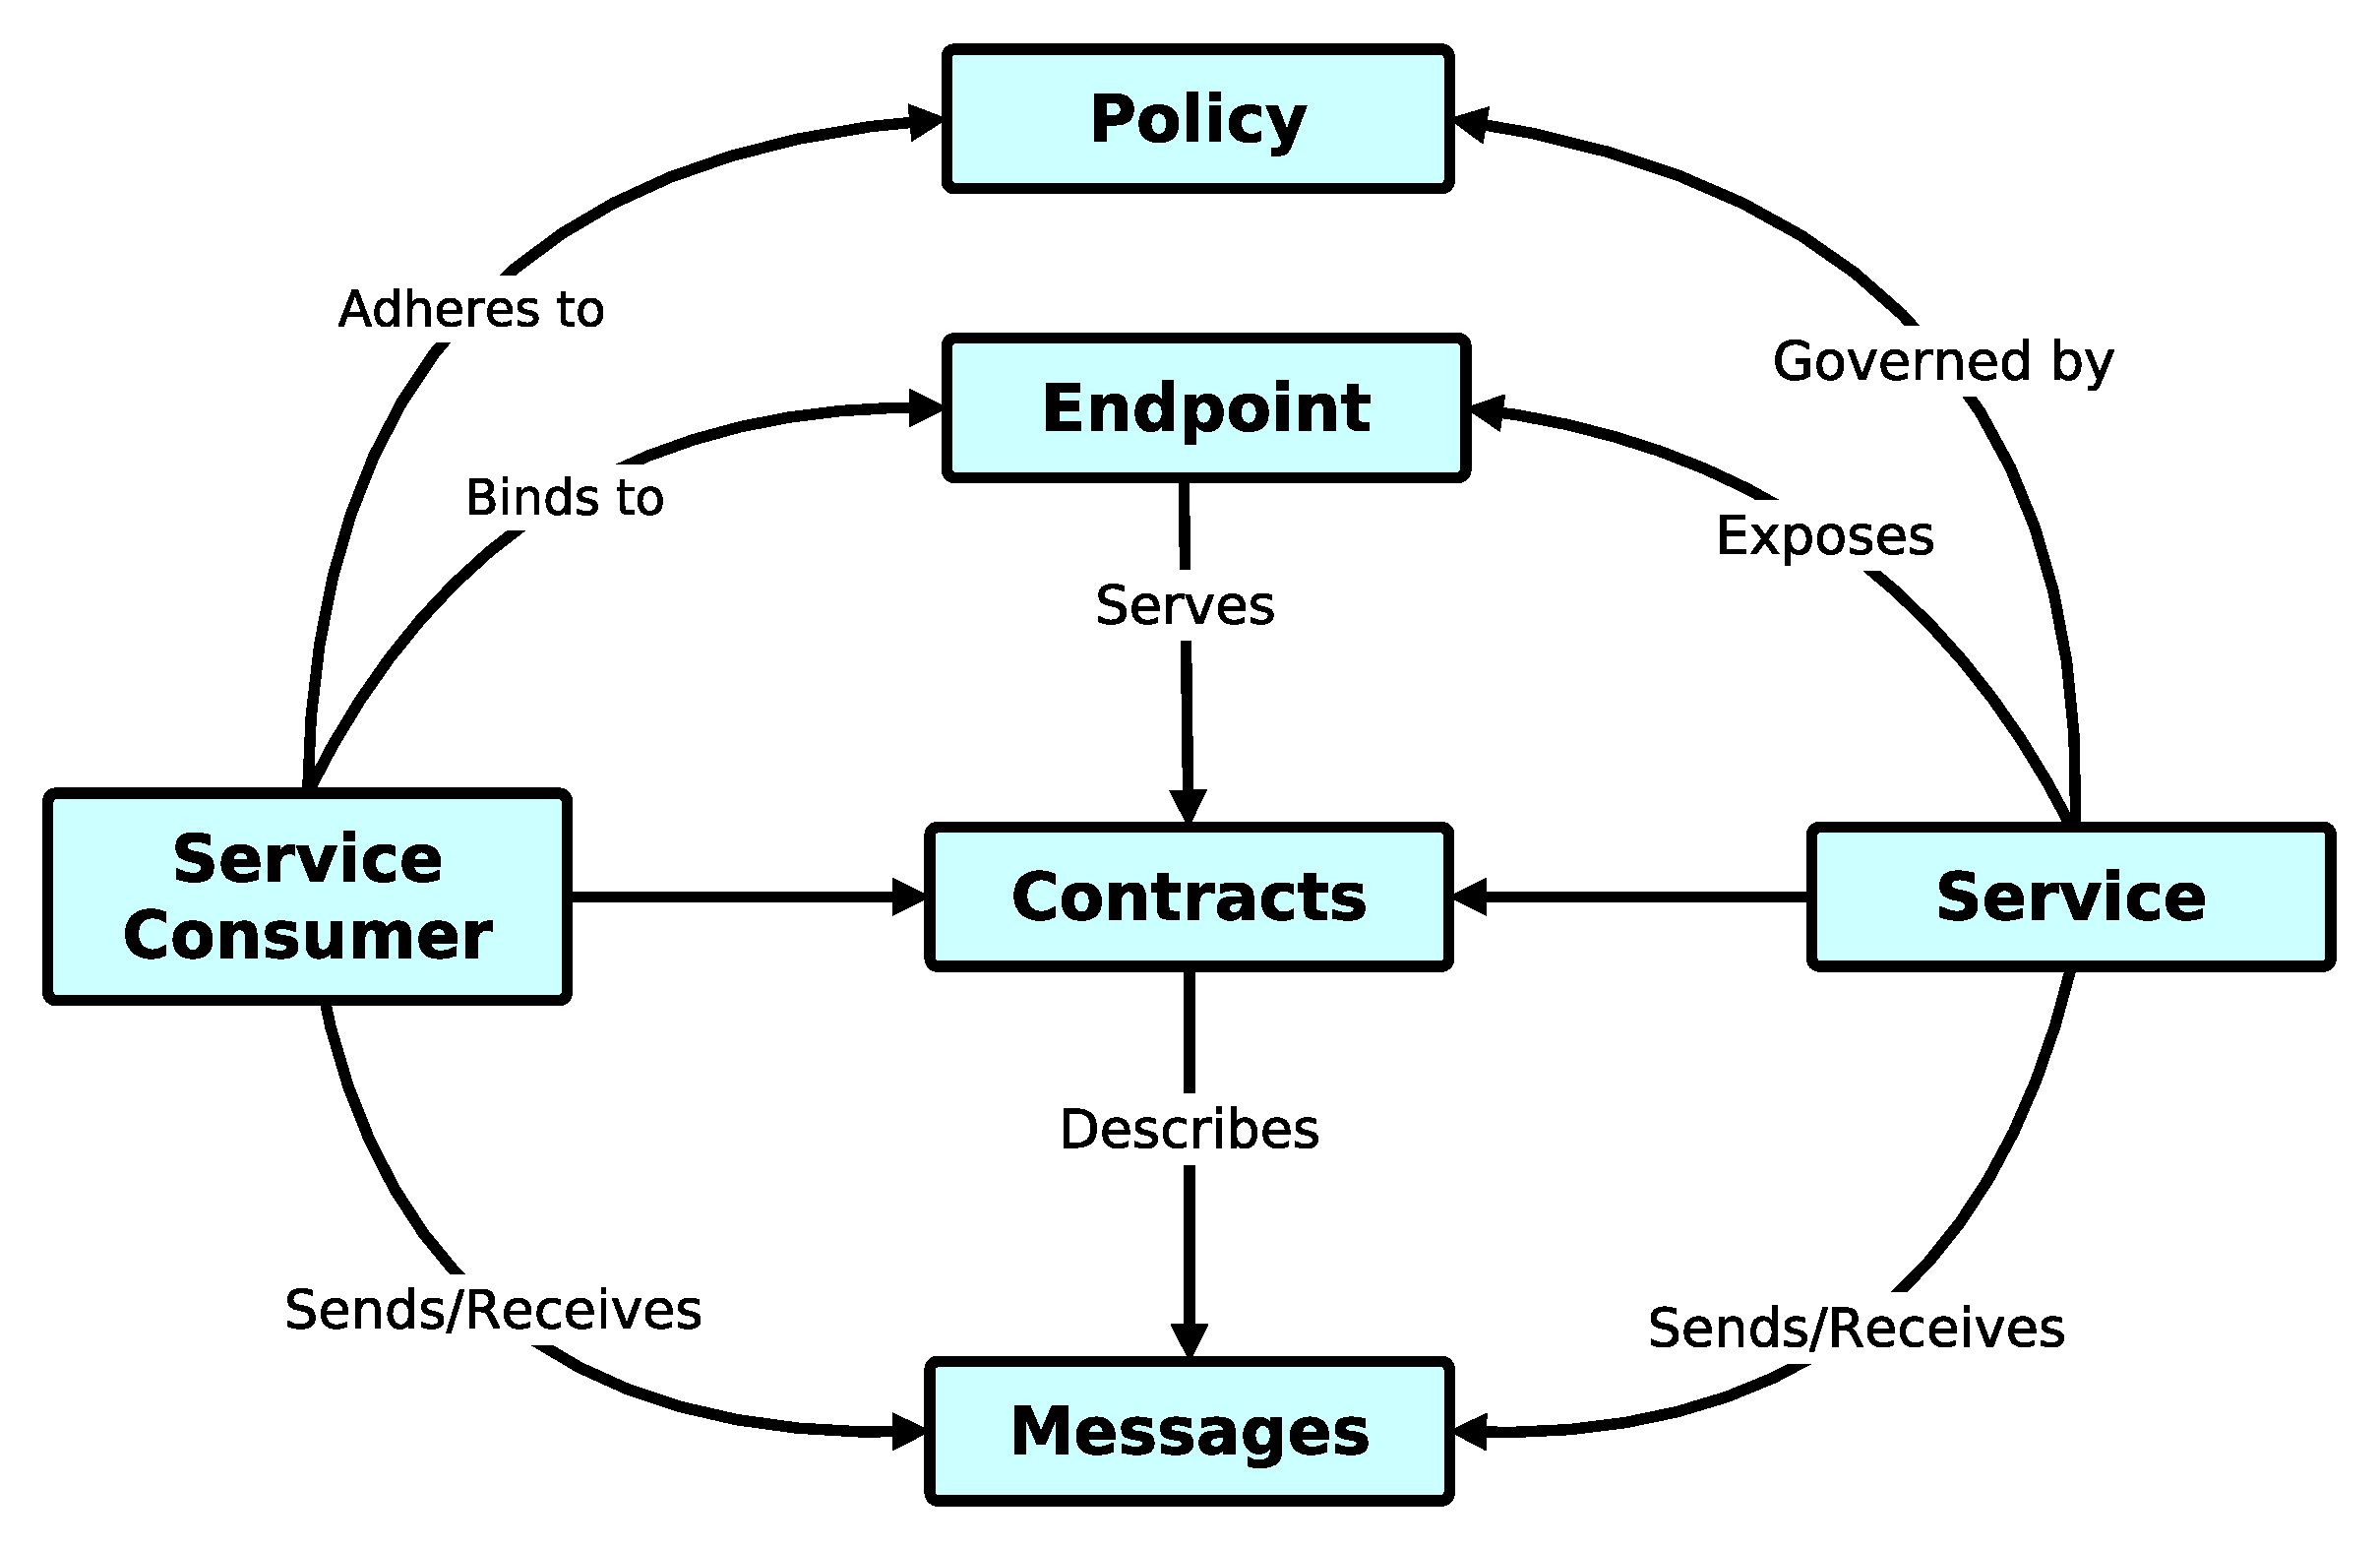
\includegraphics[scale=.2]{img/soa_relation.eps}
\caption{SOA service to consumer}
\label{fig:cm}
\end{figure}




\begin{figure}[!h]
\centering
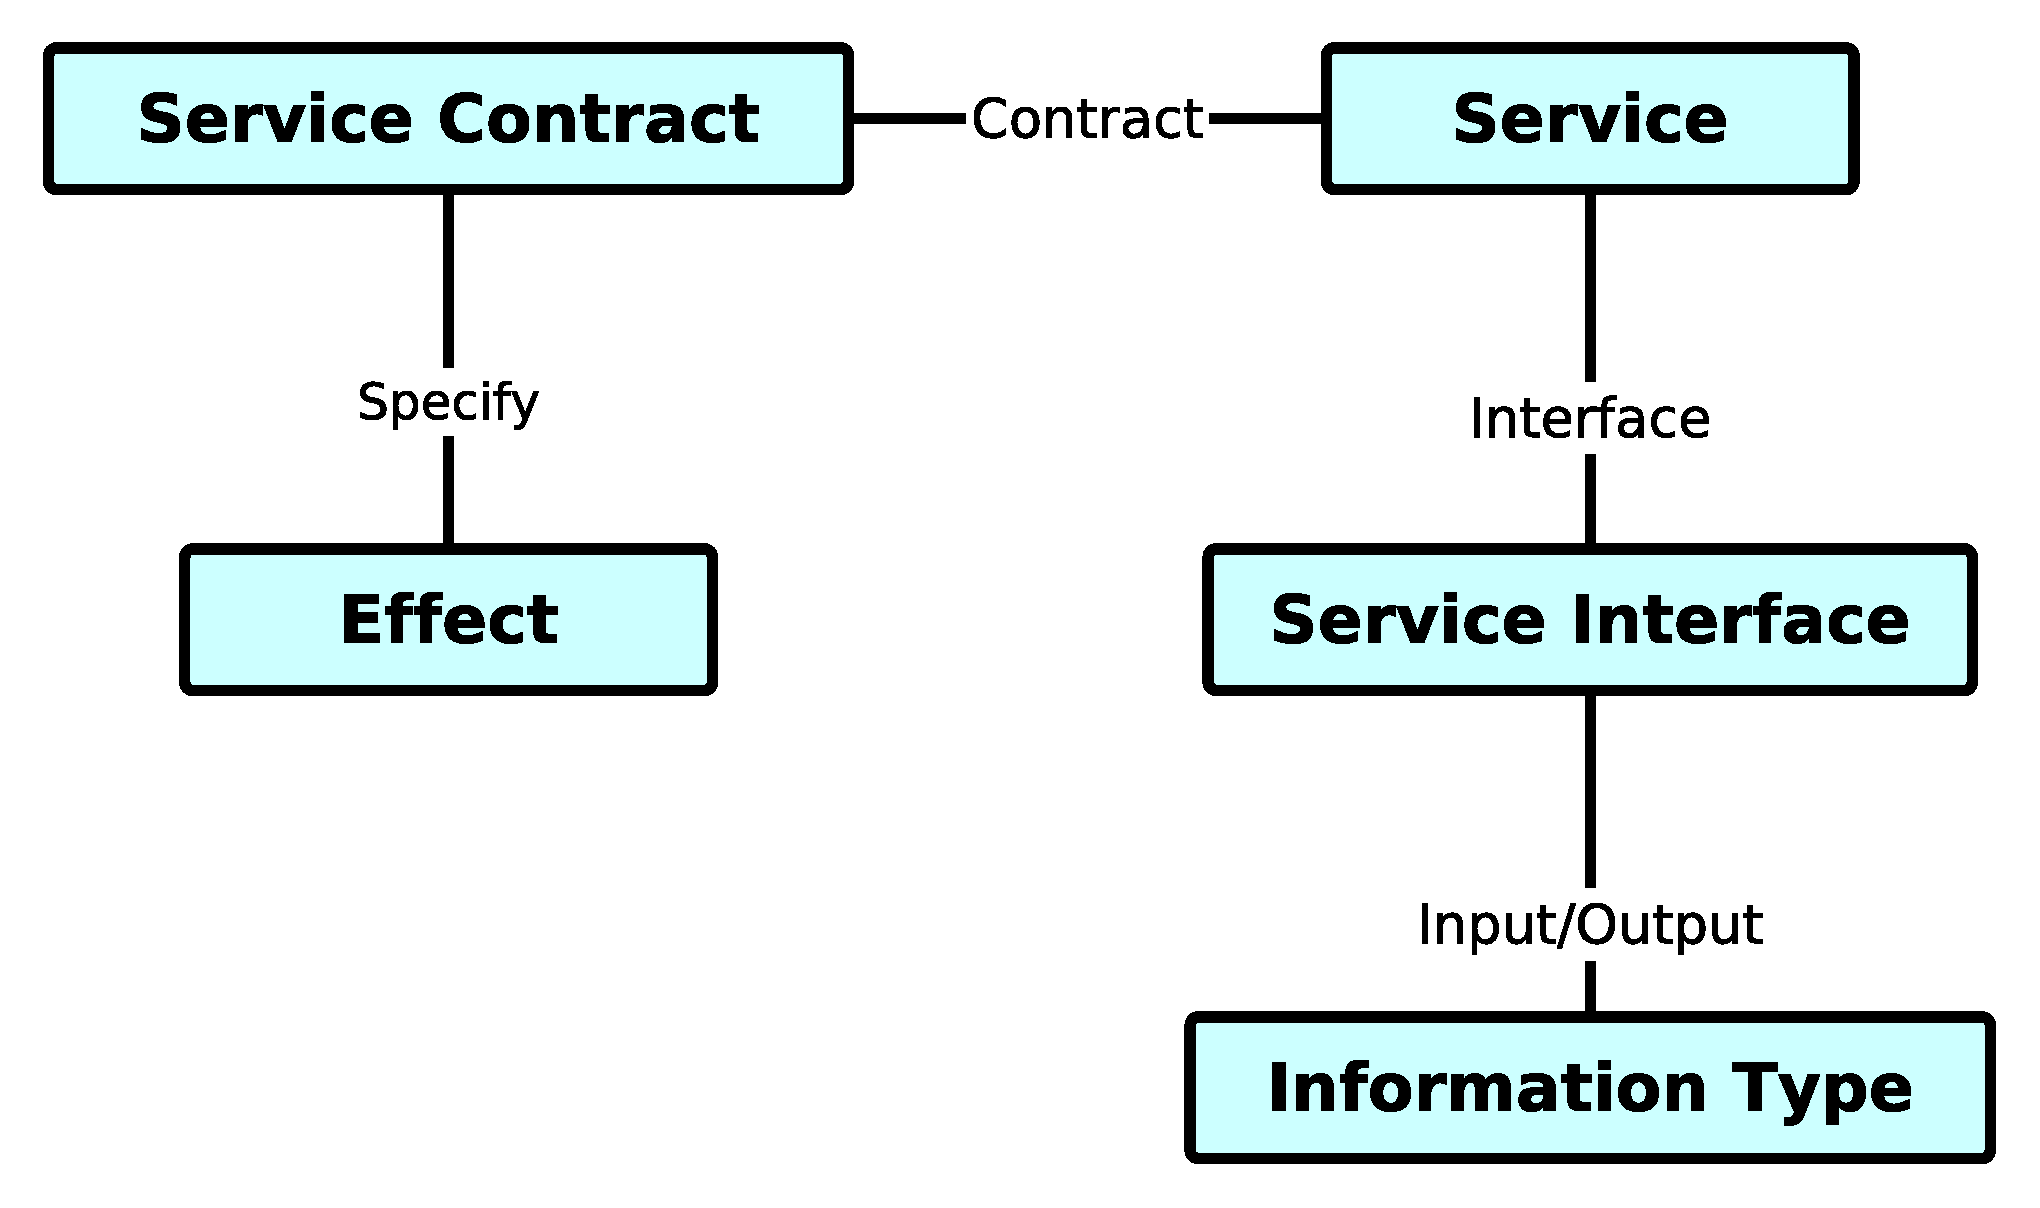
\includegraphics[scale=.2]{img/soa_property.eps}
\caption{SOA service properties}
\label{fig:cm}
\end{figure}

\subsection{Reasoning}

Deployment bez implementačních chyb.

\subsubsection{Model Integrity Validation}

Validace celého řešení vůči high level modelu.

\subsection{External Node Classification}

Mapování vybraného formátu na OpenStack

(HA architektura SDN controller)

\begin{figure}[!h]
\centering
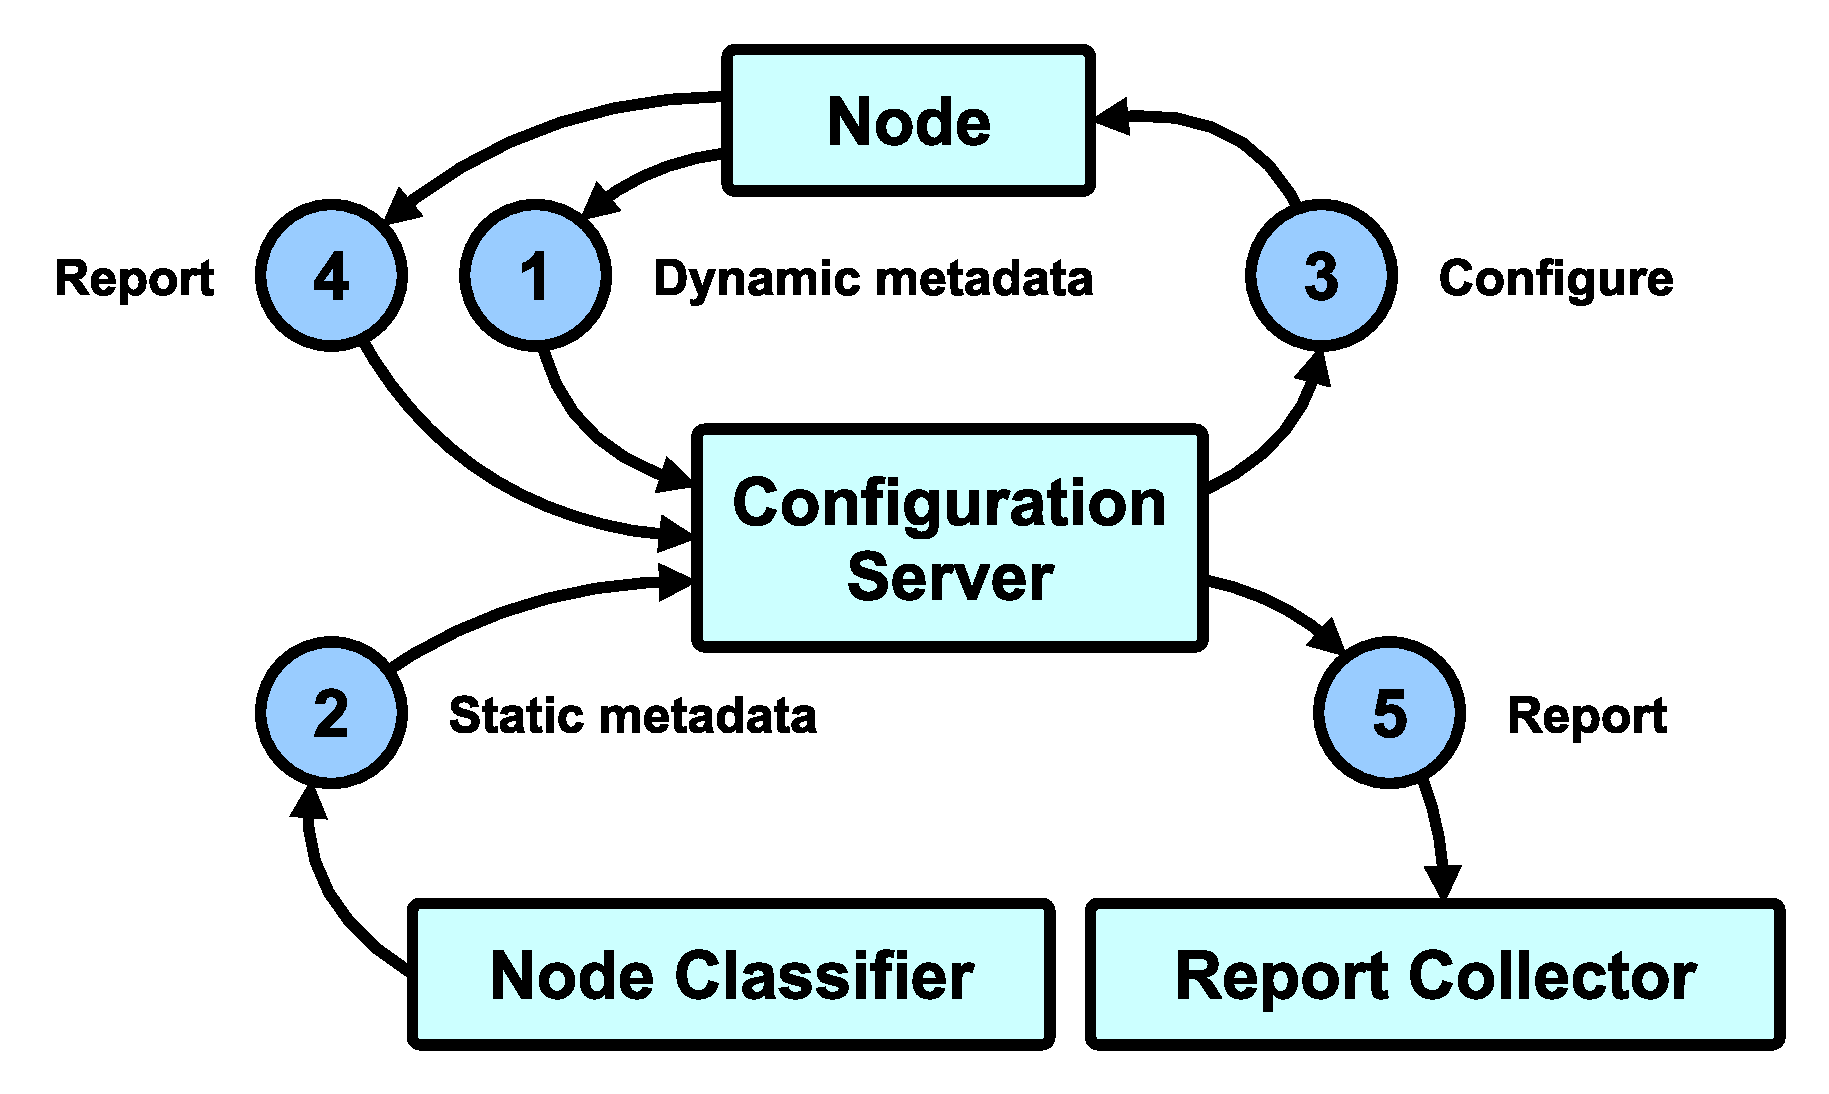
\includegraphics[scale=.15]{img/cm_cycle.eps}
\caption{Configuration Management deployment cycle}
\label{fig:cm}
\end{figure}

\subsubsection{Puppet ENC}

\subsubsection{SaltStack ENC}

Reálný přínos celého řešení
